%%%%%%%%%%%%%%%%%%%%%%%%%%%%%%%%%%%%%%%%%%%%%%%%%%%%%%%%%%%%%%%%%%%%%%
% BAB TINJAUAN PUSTAKA
%=====================================================================
\renewcommand{\thechapter}{\Roman{chapter}}
\addtocontents{toc}{\vskip10pt}
\chapter{TINJAUAN PUSTAKA}
\renewcommand{\thechapter}{\arabic{chapter}}
%---------------------------------------------------------------------

%=====================================================================
\section{Melakukan Sitasi }
%=====================================================================

Referensi berupa artikel dari jurnal ilmiah yang digunakan dalam dokumen Tugas Akhir ini, dan datanya telah dimasukkan dalam \texttt{pustaka.bib}, dapat disitasi dengan cara \citet{refJurnal} atau \citep{refJurnal}. Referensi yang digunakan juga dapat berupa artikel dari \textit{proceedings} ilmiah dan buku \citep{refProceedings,refBuku}. Referensi berupa laman internet dapat langsung dituliskan sebagai \url{https://phys.org/news/2021-11-thermoelectric-crystal-high.html} atau dengan melakukan sitasi \citep{refInternet}.

%=====================================================================
\section{Menuliskan Persamaan Matematika}
%=====================================================================

Suatu persamaan dapat dituliskan seperti contoh persamaan \textit{figure of merit} termoelektrik berikut:

\begin{equation}
    ZT = \dfrac{S^2 \sigma}{\kappa} T,
    \label{eq:persamaan1}
\end{equation}

\noindent di mana, $S$ adalah koefisien Seebeck dengan satuan V.K$^{-1}$, $\sigma$ adalah konduktivitas listrik dengan satuan S/m, $\kappa$ adalah konduktivitas panas dengan satuan W.m$^{-1}$.K$^{-1}$, dan $T$ adalah suhu termoelektrik dengan satuan K. 

Persamaan~\ref{eq:persamaan1} adalah contoh persamaan matematika dengan penomoran. Nomor persamaan pada \textit{template} \LaTeX{} Tugas Akhir ini telah diatur untuk diurutkan berdasarkan urutan kemunculan (posisi) persamaan tersebut dalam \textit{file} \texttt{$^*$.tex} dalam bagian \texttt{konten}. Untuk menuliskan persamaan tanpa penomoran dapat digunakan:

\begin{displaymath}
    \kappa = \kappa_{\rm e} + \kappa_{\rm l}
\end{displaymath}

\noindent Berbeda dengan Persamaan~\ref{eq:persamaan1}, persamaan di atas tidak memiliki nomor.


%=====================================================================
\section{Membuat Tabel}
%=====================================================================

Pada dasarnya ada berbagai tipe tabel. Tabel~\ref{tab:tabel1} adalah contoh tabel yang paling umum digunakan, yang terdiri atas 3 kolom dan 4 baris.

\begin{table}[ht] % [h] menyatakan posisi. h: here, t: top, b: bottom
	\centering
	\caption{Contoh tabel yang paling umum digunakan}
	\label{tab:tabel1}
	\begin{tabular}{c c c} % c: center, l: left (rata kiri), r: right (rata kanan)
		\hline
		Kolom-1 baris-1   & Kolom-2 baris-1   & Kolom-3 baris-1 \\
		\hline
		Kolom-1 baris-2   & Kolom-2 baris-2   & Kolom-3 baris-2 \\
		Kolom-1 baris-3   & Kolom-2 baris-3   & Kolom-3 baris-3 \\
		Kolom-1 baris-4   & Kolom-2 baris-4   & Kolom-3 baris-4 \\
		\hline
	\end{tabular}
\end{table}

\begin{sidewaystable}[h!] % [h] menyatakan posisi. h: here, t: top, b: bottom
	\centering
	\caption{Contoh tabel dengan \textit{multicolumn} dan \textit{multirow}}
	\label{tab:multitab}
	\begin{tabular}{l c c r} % c: center, l: left (rata kiri), r: right (rata kanan)
		\hline
		\multirow{2}{*}{Kol-1 baris-1/2}  & \multicolumn{2}{c}{Kol-2/3 baris 1}  & \multirow{2}{*}{Kol-4 baris-1/2} \\
		                                  & Kol-2 baris-2                        & Kol-3 baris-2   & \\
		\hline
		Kol-1 baris-3  & Kol-2 baris-3    & Kol-3 baris-3   & Kol-4 baris-3 \\
		Kol-1 baris-4  & Kol-2 baris-4    & Kol-3 baris-4   & \multirow{2}{*}{Kol-4 baris-4/5} \\
		Kol-1 baris-5  & $^*$Kol-2 baris-5    & $^{**}$Kol-3 baris-5   & \\		                                  
		\hline
		\multicolumn{4}{r}{$^*$\citealt{refJurnal}} \\ % Contoh sitasi catatan kaki
		\multicolumn{4}{r}{$^{**}$\citealt{refProceedings}} % Contoh sitasi catatan kaki
	\end{tabular}
\end{sidewaystable}

Sementara itu, Tabel~\ref{tab:multitab} adalah contoh tabel \textit{landscape} yang menggunakan \textit{multicolumn} dan \textit{multirow}, yang pada dasarnya terdiri dari 4 kolom dan 5 baris.

\newpage % Untuk melanjutkan bagian di bawah ini pada halaman baru
%---------------------------------------------------------------------
\subsection{Memasukkan Gambar dan Kode}
%---------------------------------------------------------------------

\textit{File} gambar perlu diunggah terlebih dahulu ke dalam folder \texttt{gambar}. Keterangan Gambar~\ref{fig:gambar1} dapat dituliskan pada \texttt{caption}.

\begin{figure}[h] % [h] menyatakan posisi. h: here, t: top, b: bottom
    \centering
    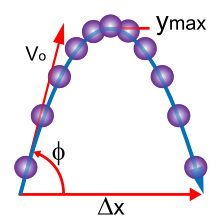
\includegraphics[width=5cm]{./gambar/contoh.png}
    \caption{Keterangan gambar dapat dituliskan di sini.}
    \label{fig:gambar1}
\end{figure}

Apabila mahasiswa/(i) perlu untuk menampilkan kode, \textit{script} program atau sejenisnya, contoh di bawah ini dapat digunakan sebagai acuan.

{\color{blue}
\begin{lstlisting}
sudo apt install build-essential g++ gfortran 
sudo apt install libblas-dev liblapack-dev 
    libopenmpi-dev libscalapack-mpi-dev 
\end{lstlisting}
}


%---------------------------------------------------------------------
\subsection{Memuat kode ringkas dari simbol, satuan, dan singkatan}
%---------------------------------------------------------------------

Untuk memuat kode ringkas dari simbol, satuan, dan singkatan yang telah dinyatakan dalam \texttt{kodeUnit.tex}, sebagai contoh, dapat dilakukan dengan \schro{} atau \its. Kode tersebut dapat diubah dan kode lain dapat ditambahkan pada \texttt{kodeUnit.tex}.

\newpage
%---------------------------------------------------------------------
\subsection{Daftar kode untuk simbol matematika dan Yunani}
%---------------------------------------------------------------------

\begin{tabular}{l l}
$\leq$ &  $\backslash$leq \\
$\geq$ &  $\backslash$geq \\
$\neq$ &  $\backslash$neq \\
$\nleq$ &  $\backslash$nleq \\
$\ngeq$ &  $\backslash$ngeq \\
$\cong$ &  $\backslash$cong \\
$\equiv$ &  $\backslash$equiv \\
$\sim$ &  $\backslash$sim \\
$\approx$ &  $\backslash$approx \\
$\times$ &  $\backslash$times \\
$\cdot $ &  $\backslash$cdot \\
$\ast $ &  $\backslash$ast \\
$\div$ &  $\backslash$div \\
$\pm$ &  $\backslash$pm \\
$\mp$ &  $\backslash$mp \\
$\oplus$ &  $\backslash$oplus \\
$\otimes$ &  $\backslash$otimes \\
$\propto $ &  $\backslash$propto \\
$\infty$ & $\backslash$infty \\
$\because$ &  $\backslash$because \\
$\therefore$ &  $\backslash$therefore \\
\end{tabular}
\hspace*{1ex}
\begin{tabular}{ll}
$\in$ &  $\backslash$in \\
$\subset $ &  $\backslash$subset \\
$\subseteq $ &  $\backslash$subseteq \\
$\varnothing $ &  $\backslash$varnothing  \\
$\cap $ &  $\backslash$cap \\
$\cup $ &  $\backslash$cup \\
$\Rightarrow$ &  $\backslash$Rightarrow \\
$\rightarrow$ &  $\backslash$rightarrow \\
$\partial$ &  $\backslash$partial \\
$90^\circ$ &  90$^\wedge\backslash$circ \\
$\parallel$ &  $\backslash$parallel \\
$\bot$ &  $\backslash$bot \\
$\triangle$ &  $\backslash$triangle \\
$\nabla$ &   $\backslash$nabla \\
$\angle$ &  $\backslash$angle \\
$\Pi$ &  $\backslash$Pi \\
$\Theta$ &  $\backslash$Theta \\
$\Gamma$ &  $\backslash$Gamma \\
$\Delta$ &  $\backslash$Delta \\
$\Omega$ &  $\backslash$Omega \\
$\Sigma$ &  $\backslash$Sigma \\
\end{tabular}
\hspace*{1ex}
\begin{tabular}{l l}
\& & $\backslash$\& \\
\% & $\backslash$\% \\
$\alpha$ &  $\backslash$alpha \\
$\beta$ &  $\backslash$beta \\
$\epsilon$ &  $\backslash$epsilon \\
$\zeta$ &  $\backslash$zeta \\
$\eta$ &  $\backslash$eta \\
$\kappa$ &  $\backslash$kappa \\
$\lambda$ &  $\backslash$lambda \\
$\mu$ &  $\backslash$mu \\
$\xi$ &  $\backslash$xi \\
$\rho$ &  $\backslash$rho \\
$\tau$ &  $\backslash$tau \\
$\phi$ &  $\backslash$phi \\
$\psi$ &  $\backslash$psi \\
$\pi$ &  $\backslash$pi \\
$\theta$ &  $\backslash$theta \\
$\gamma$ &  $\backslash$gamma\\
$\delta$ &  $\backslash$delta \\
$\omega$ &  $\backslash$omega \\
$\sigma$ &  $\backslash$sigma \\
\end{tabular}
 

\newpage
